\documentclass{standalone}
\usepackage{tikz}


% w_0 = xy
% w_1 = w_0 + x
% z = sin w_1
% 
% z' = dz/dz = 1
% w1' = w2' * cos w1
% w0' = w1' * 1
% x'_1 = w1'*1
% x'_2 = w0'*y
% y' = w1'*x
% 
% x' = w0'*x = w1'*x = (w2'*cos w1)*x = 1*cos(xy+x)*y = cos(xy+x)*y + cos(xy+x) = cos(xy+x)*(y + 1)
% y' = w1'*x = w2'*(cos w1)*x = 1*(cos (xy + x))*x


\begin{document}
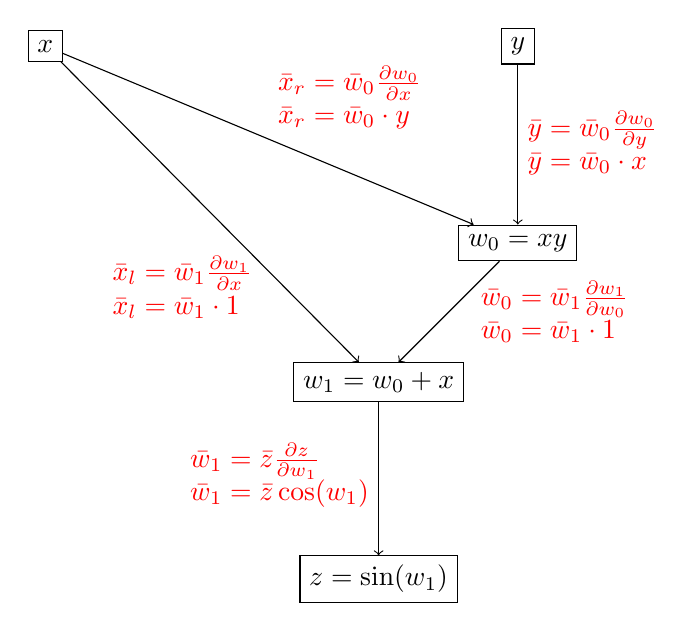
\begin{tikzpicture}[node distance=2.5cm]

    % Nodes
    \node (x) [draw] {$x$};
    \node (y) [draw, node distance=6cm, right of=x] {$y$};
    \node (w0) [draw, below of=y] {$w_0 = xy$};
    \node (w1) [draw, below left of=w0] {$w_1 = w_0 + x$};
    \node (w2) [draw, below of=w1] {$z = \sin(w_1)$};

    % Arrows
    \draw[->] (x) -- (w0)
              node[midway,above right,text=red,align=left] 
              { $\bar{x}_r = \bar{w}_0\frac{\partial w_0}{\partial x}$\\
                $\bar{x}_r = \bar{w}_0\cdot y$
              };
    \draw[->] (y) -- (w0)
              node[near end,above right,text=red,align=left] 
              { $\bar{y} = \bar{w}_0\frac{\partial w_0}{\partial y}$\\
                $\bar{y} = \bar{w}_0\cdot x$
              };
    \draw[->] (w0) -- (w1)
              node[midway,right=8,text=red,align=left] 
              { $\bar{w}_0 = \bar{w}_1\frac{\partial w_1}{\partial w_0}$\\
                $\bar{w}_0 = \bar{w}_1\cdot 1$
              };
    \draw[->] (x) --  (w1)
              node[near end,left=8,text=red,align=left] 
              { $\bar{x}_l = \bar{w}_1\frac{\partial w_1}{\partial x}$\\
                $\bar{x}_l = \bar{w}_1\cdot1$
              };
    \draw[->] (w1) -- (w2) 
              node[near end,above left,text=red,align=left] 
              { $\bar{w}_1 = \bar{z}\frac{\partial z}{\partial w_1}$\\
                $\bar{w}_1 = \bar{z}\cos(w_1)$
              };

\end{tikzpicture}
\end{document}



